% Syslab Research Journal Template
% By Patrick White
% September 2019

% Do not edit this header
\documentclass[letterpaper,11pt]{article}
\usepackage{fullpage}
\usepackage{palatino}
\usepackage{enumitem}
\usepackage{courier}
\usepackage{graphicx}
\def\hrulefill{\leavevmode\leaders\hrule height 20pt\hfill\kern\z@}

% ------------- Edit these definitions ---------------------
\def\name{Bryan Lu}
\def\journalnum{14}
\def\daterange{01/13/20-01/20/20} % starts on Monday
\def\period{2}
% ------------------ END ---------------------------------
% Do not edit this
\begin{document}
	\thispagestyle{empty}
	\begin{flushright}
		{\Large Journal Report \journalnum} \\
		\daterange\\
		\name \\
		Computer Systems Research Lab \\
		Period \period, White
		\end{flushright}
	\hrule height 1pt

% ------ SECTION DAILY LOG -------------------------------------
\vspace{-0.8em}
\section*{Daily Log}
%Detail for each day about what you research, coded, debug, designed, created, etc. Informal style is OK.
\vspace{-0.8em}
\subsection*{Monday, January 13}
\vspace{-0.6em}
Figured out the correct arguments to pass through to the parser, got code to work up until a request to a local server, presumably a Stanford NLP server. 
 
\vspace{-1.3em}
\subsection*{Tuesday, January 14}
\vspace{-0.6em}
Consulted Dr. White with what to do about the Stanford server, installed the server on my computer, and successfully obtained a  connection to the server and received data from it. 

\vspace{-1.3em}
\subsection*{Thursday, January 16}
\vspace{-0.6em}
Played with Stanford server with small sentences, figured out the right request to reliably return data, but not the data that I needed for the code. 

\vspace{-0.8em}

% ------ SECTION TIMELINE -------------------------------------
%\newpage
%\vspace{-1.7em}
\vspace{-1.0em}
\section*{Timeline}
\begin{tabular}{|p{1in}|p{2.5in}|p{2.5in}|}
	\hline
\textbf{Date} & \textbf{Goal} & \textbf{Met}\\ \hline 
	\hline
1/6 & Figure out what the best next steps are for moving forward, based on not quite reaching my winter goal. & I think I have a fairly concrete plan for what to work on moving forward, but I'm not sure if it's super feasible\ldots need to discuss still. \\
	\hline 
1/13 & Get a script heavily based on their code to be runnable, pending annotations. & Almost, I just need one last push to get the last piece of the code in the syntax parsing to work. \\
	\hline 
1/20 & Adapt the question input for their code to access local files instead of a database, try running their code with olympiad problems. & N/A \\
	\hline 
1/27 & Pending annotations, get everything up until the annotations step to work with olympiad problems, and work out other cosmetic details. & N/A \\
	\hline
\end{tabular}

\pagebreak 
% ------ SECTION REFLECTION  ---------------------------------
\section*{Reflection}
%In narrative style, talk about your work this week. Successes, failures, changes to timeline, goals. This should also include concrete data, e.g. snippets of code, screenshots, output, analysis, graphs, etc.

I felt I was pretty productive this week -- I'm currently working on running a snippet of code to process one of the questions in their provided testcases set to figure out what sort of structure their ``syntax parses'' are for each question, i.e. the data about words in each of the sentences for each question. 

I finally had to configure the Stanford NLP parsing server that the paper mentioned, and I think I got it to work pretty successfully! As a proof of concept, here's an example of the Stanford parser server running on an actual sentence. This one is a bit longer than the one I've been using all week, but it's to show that it can handle long sentences just fine. This is the final quote from Dickens' \textit{A Tale of Two Cities}, and the parser server returns part-of-speech tags and the dependency relations between different words: 
\begin{center}
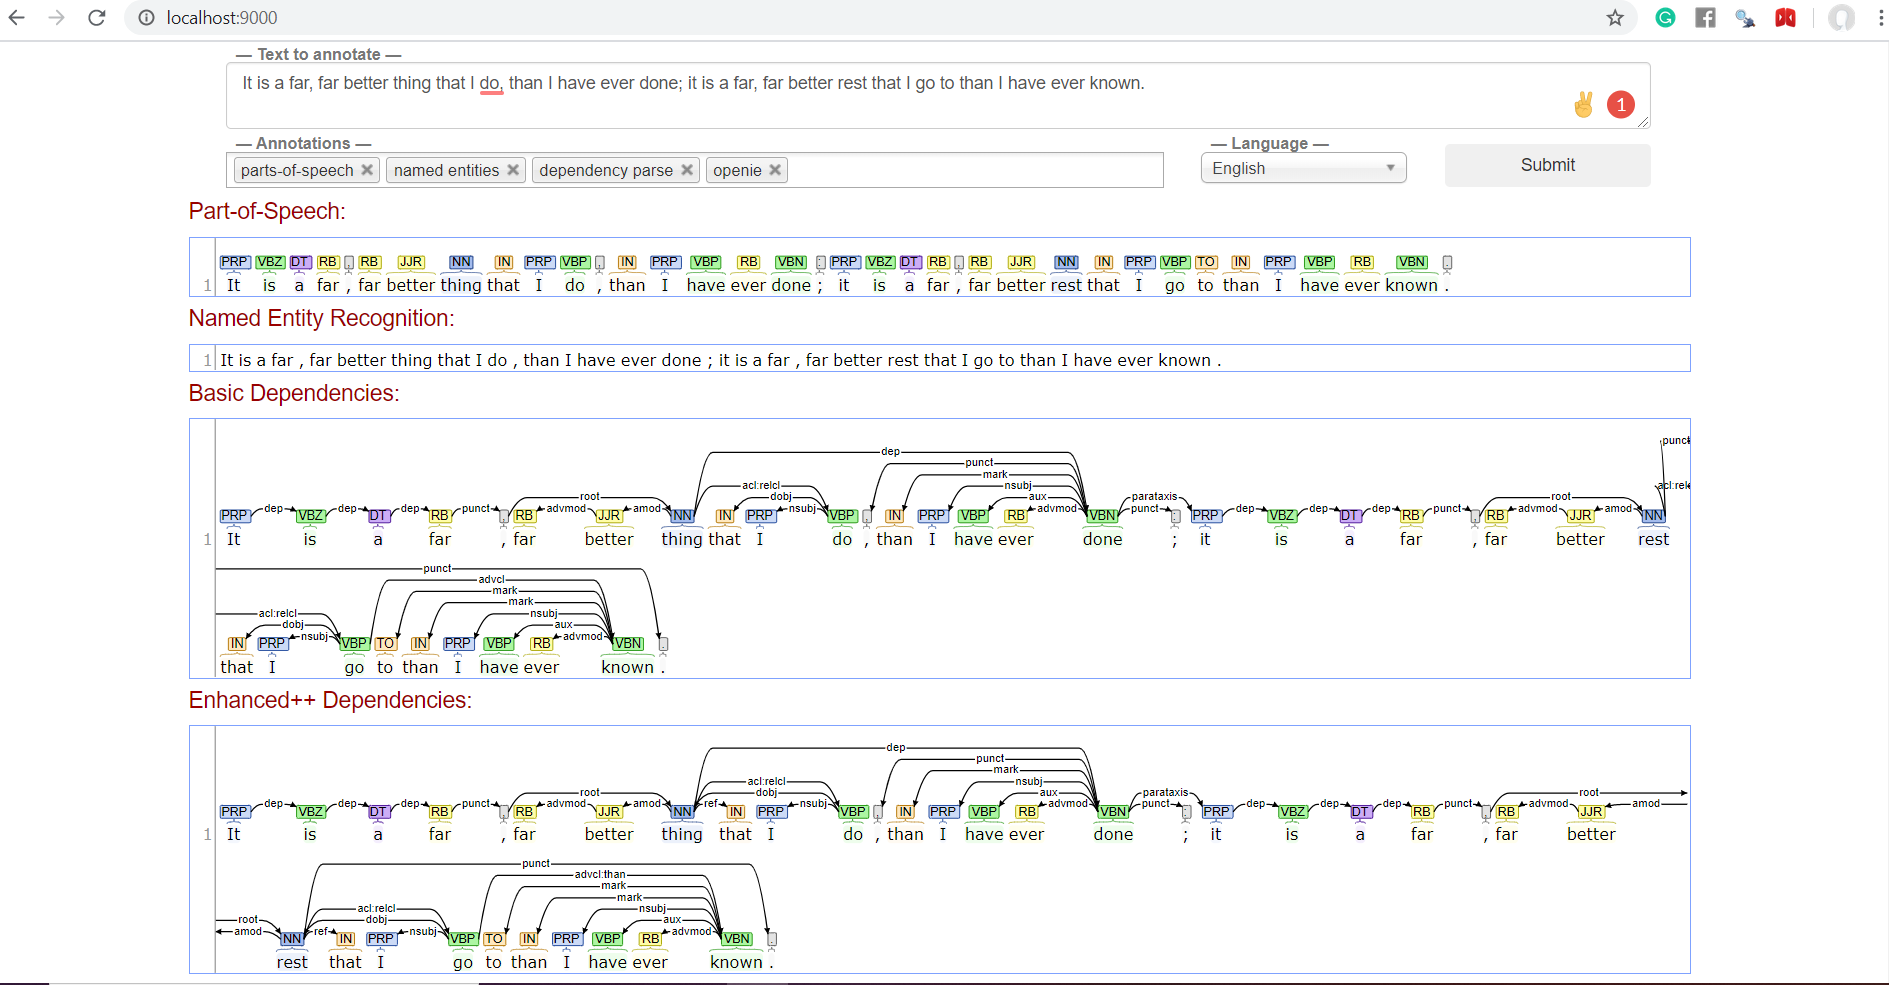
\includegraphics[scale=0.4]{stanford.png}
\end{center}
This is a good step as eventually I'm going to need this information when I deal with individual questions. 

Obviously, the server does other things, but I've not been patient enough/haven't properly figured out what they are and what they do. What's left for me to figure out is what function is being run on the server so that the last bit of data processing works, because in these two lines of code: 
\begin{center}
\texttt{score = tree\_data['score']}\\
\texttt{tuples = tree\_data['tuples']}
\end{center}
they seem to be accessing \texttt{score} and \texttt{tuples} keys in the returned dictionary, and I'm not currently aware of how these keys can be made. 

\end{document}

